\section{Four additional signals and their limitations}
\label{sec:other}

The remaining four signals illustrate distinct obstacles: a deep event with
ambiguous companion size, two shallow signals with inadequate predictive timing,
and recurring dimming for which a resolved neighboring binary is a plausible
source. All measurements below retain the historical clocks and unfavorable
alternatives. Formal errors describe the stated measurement model; they omit
some correlated noise, timing and source uncertainties. Repeated reductions of
one sector do not constitute independent observations.

\subsection{TIC 241928959: target-region dimming with physical degeneracies}
\label{sec:tic241}
% Evidence: results/qlp-faint-midradius-single-review-20261011/241928959-peak0/ASSESSMENT.md
% results/event-baseline-six-20261012/ASSESSMENT.md

The approximately 3.533-day pattern is measured in sector 92 alone. Its refined
training clock is $P=3.532592898$~d with a 0.032-day box duration. Five usable,
discovery-selected events give an event-baseline depth of $11\,992\pm786$~ppm;
removing each event in turn leaves $11\,729$--$12\,442$~ppm. One disturbed event
remains excluded because its in-window samples carry nonzero quality flags and
lack a usable baseline. The 2.5-day detrending removes another event's
in-transit samples, leaving four observed transits. The physical fitter's six
local windows include baseline-only windows and must not be counted as six
transits. The deeper final event remains in the analysis.

% Evidence: results/prf-fullscene-241928959-20261011/ASSESSMENT.md
% results/prf-events-241928959-20261011/ASSESSMENT.md
Difference images favor the target region over TIC 241928961, a neighbor
10.56~arcsec away. A fuller scene model gives $\chi^2=109.16$ for the target
and 437.05 for that neighbor, each with 117 degrees of freedom. All five
individual events and their omission stacks prefer the target in the original
brighter-scene model. These conditional template comparisons do not exclude
unresolved companions or calibrate host probabilities. An illustrative
equal-throughput blend with the known neighbor would require a roughly
24\% eclipse; the actual aperture response is not known.

% Evidence: results/physical-241928959-20261012/ASSESSMENT.md
The short shape does not provide a secure companion radius
(Figure~\ref{fig:241physical}). For the 1.5-day reduction, a circular,
undiluted target model with freely fitted $a/R_\star$ gives radius ratio
$k=0.1257$, impact parameter $b=0.840$ and an inferred stellar density
$15.66~\mathrm{g\,cm^{-3}}$. The nominal catalog mass and radius imply only
about $3.21~\mathrm{g\,cm^{-3}}$. A broad prior on $a/R_\star$ instead permits
$k=0.3072$ and $b=1.135$, a grazing configuration, at a data-fit cost of only
$\Delta\chi^2\simeq1.7$. The second detrending retains this degeneracy.
Eccentricity, dilution and stellar-model errors remain unmodeled alternatives.
The restricted neighbor fit reaches its upper radius-ratio bound; it is not a
general eclipsing-binary exclusion.

% Evidence: results/companion-constraints-shortlist-20261012/ASSESSMENT.md
% results/parity-241928959-20261011/ASSESSMENT.md
% results/secondary-241928959-20261011/ASSESSMENT.md
% results/coverage-review-241928959-20261011/ASSESSMENT.md
Gaia RUWE 3.356 and a 14\% multiple-peak image fraction reinforce caution about
a single-star interpretation, without demonstrating a companion. Alternating
depths differ by less than one formal standard deviation, but only one usable
odd-family event is available. Fixed half-phase tests find no convincing
secondary eclipse and do not exclude an eccentric or faint binary. Existing
ZTF measurements are inconclusive, and the checked TESS coverage supplies no
verified second observing epoch. Source identity, companion size and recurrence
therefore remain unresolved.

\begin{figure}[p]
\centering
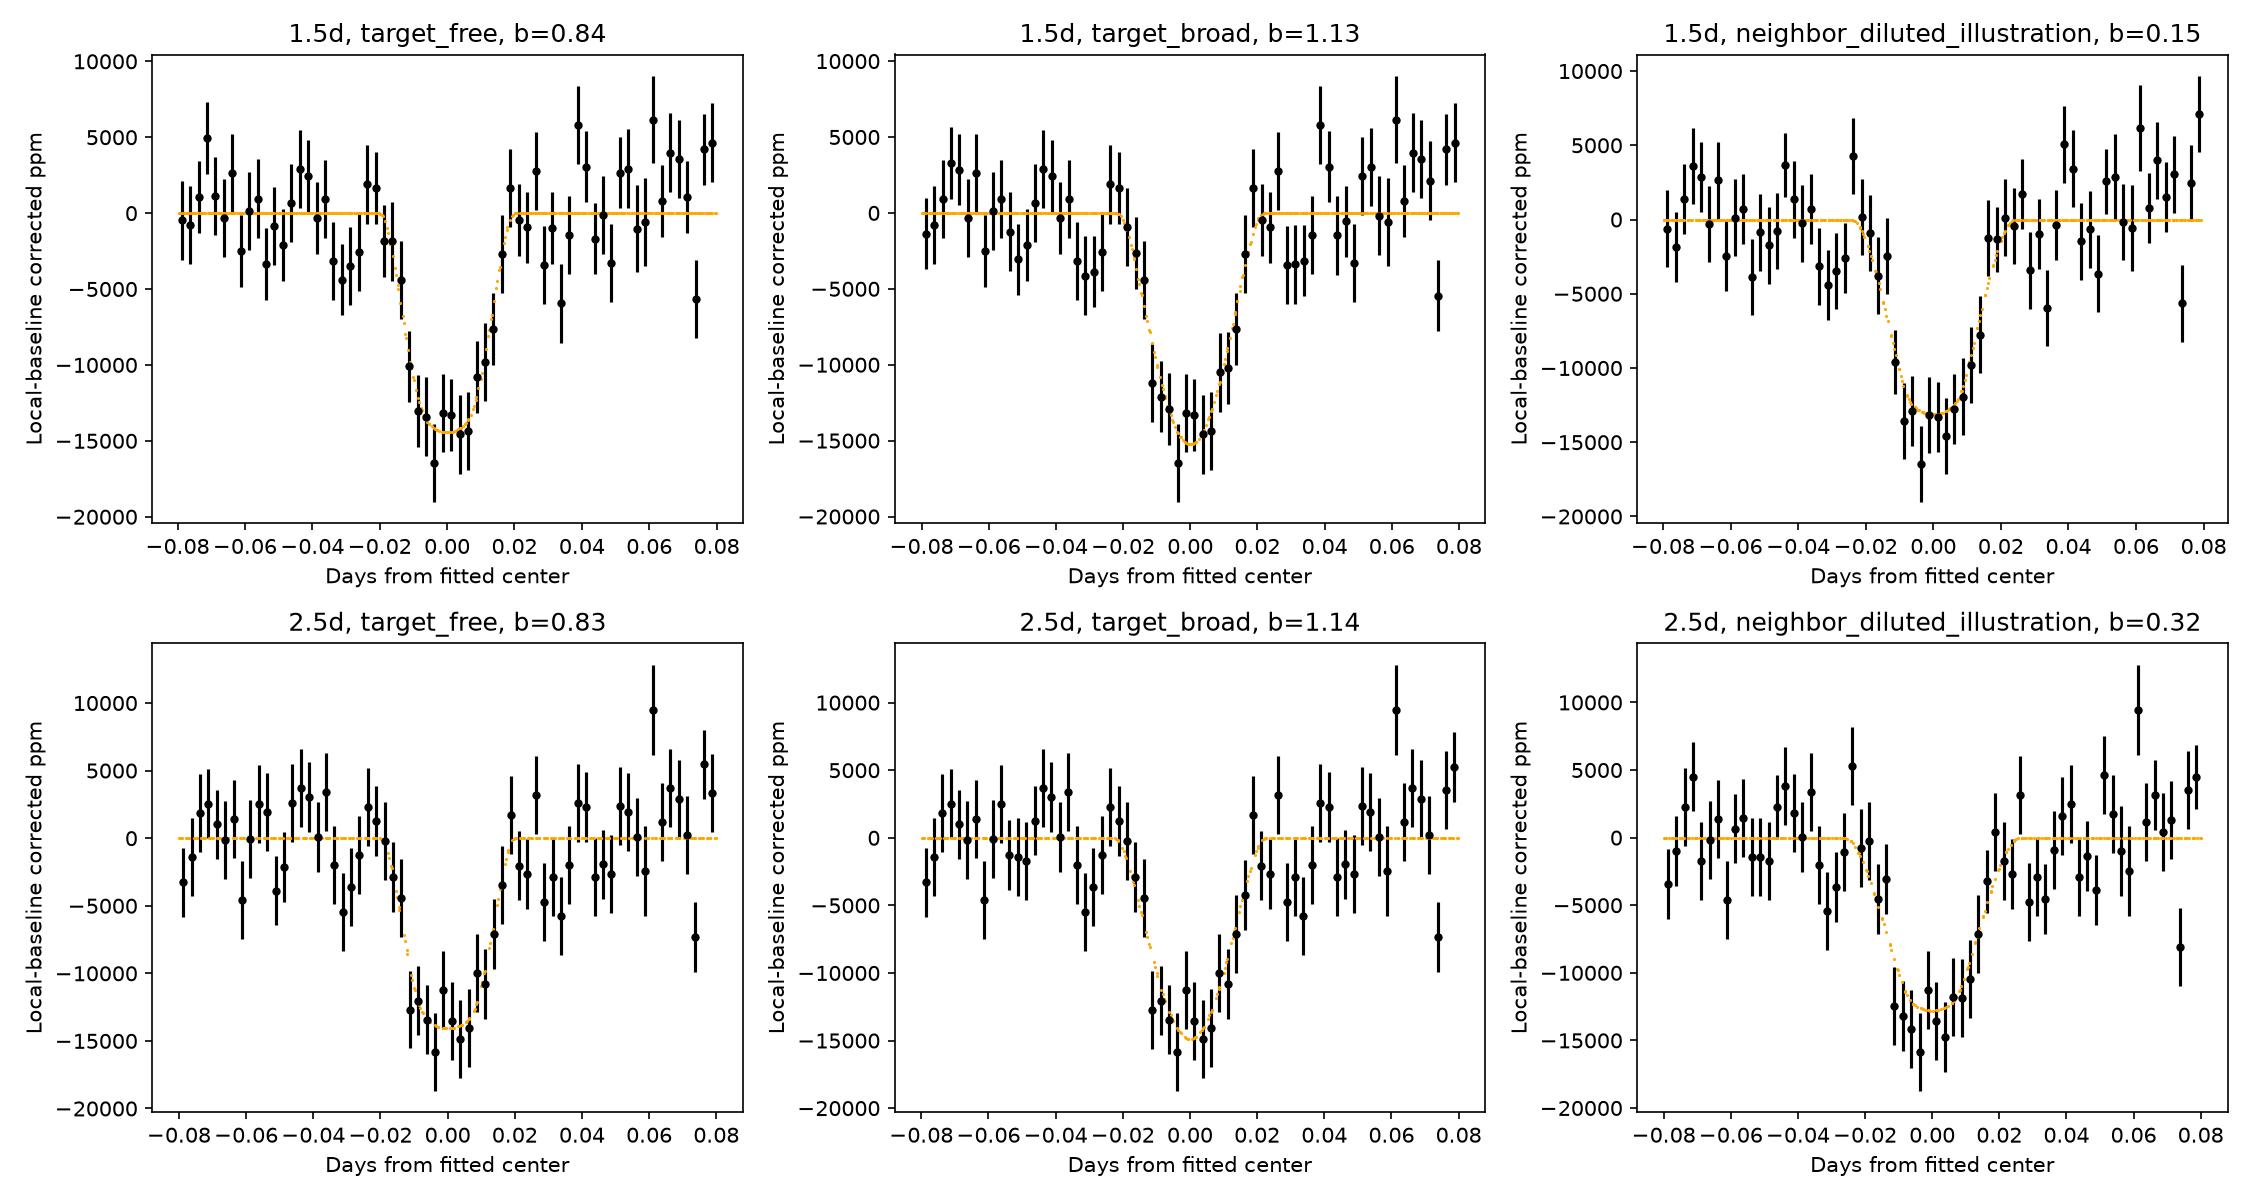
\includegraphics[width=\linewidth]{figures/241-physical.png}
\caption{Conditional physical fits to the same sector-92 observations of
TIC 241928959. Rows use the 1.5- and 2.5-day detrending windows; columns show
a target model with free orbital scale, a target model with a broad scale
prior, and an illustrative diluted-neighbor model. Similar folded shapes
accommodate very different companion sizes and grazing geometries. The neighbor
model reaches its radius-ratio bound and does not span general stellar-eclipse
models. These fits supply no independently validated planet radius.}
\label{fig:241physical}
\end{figure}

\subsection{TIC 469309982: mixed recurrence and a seasonal secondary concern}
\label{sec:tic469}
% Evidence: results/followup-469309982-20261011/ASSESSMENT.md
% results/season-out-469309982-20261011/ASSESSMENT.md

The four-sector weak-seed refinement uses sectors 9, 10, 36 and 37 and selects
$P=2.890464274$~d, a 0.144-day duration and a fitted depth of 138~ppm. Sector 64
at the unchanged nominal clock gives $75.8\pm26.2$~ppm. Its propagated timing
spread, 0.12347~d, exceeds the allowed half-duration of 0.072~d. A previously
saved alternative gives $133.4\pm26.2$~ppm, but this maximum across nine
correlated clocks cannot replace the nominal prediction. Sector 63, evaluated
using the clock selected after examining sector 64, is also weak:
$82\pm28$~ppm, falling to 21~ppm when one event is omitted.

Only one of six retrospective season-out comparisons passes both the original
recovery and timing conditions: the 1.5-day detrending predicts the omitted
sectors 36/37 at $129.7\pm22.6$~ppm with a 0.0525-day timing spread
(Figure~\ref{fig:469seasons}). The corresponding 2.5-day result is positive,
$136.7\pm23.5$~ppm, but separated accepted aliases expand its spread to
1.5706~d. All observations were previously inspected, the folds overlap, and
the discovery seed uses sectors 9/10 even when that season is omitted.

% Evidence: results/secondary-seasons-469309982-20261011/ASSESSMENT.md
% results/prf-motion-469309982-20261011/ASSESSMENT.md
A possible half-phase secondary is concentrated in sectors 36/37:
$87.8\pm22.7$~ppm at the 1.5-day window, compared with $24.0\pm22.6$ and
$-0.5\pm19.7$~ppm in the earlier and later seasons. This remains a concern
rather than a repeatable binary eclipse. Image models often favor neighbor
TIC 469309967, but substantial residuals and failures on known-planet controls
prevent a reliable source assignment.

% Evidence: results/new-epochs-469309982-96166003-20261012/ASSESSMENT.md
Sector 90 gives $-54.3\pm31.6$~ppm at the primary refined clock and
$14.1\pm33.8$~ppm at the alternate refined clock. Positive measurements at
the original unprofiled seed are retained without substitution
(Figure~\ref{fig:469961new}). Timing is inadequate and expected formal
sensitivity is below $5\sigma$, so this does not establish either recovery or
exclusion. The exact-source open-cluster reference supplies no useful age
prior.\footnote{TIC 469309982 is HD 300413. Its row in the checked Platais 8
membership table reports membership probability 0.00; bibliographic inclusion
is not cluster membership.}

\begin{figure}[p]
\centering
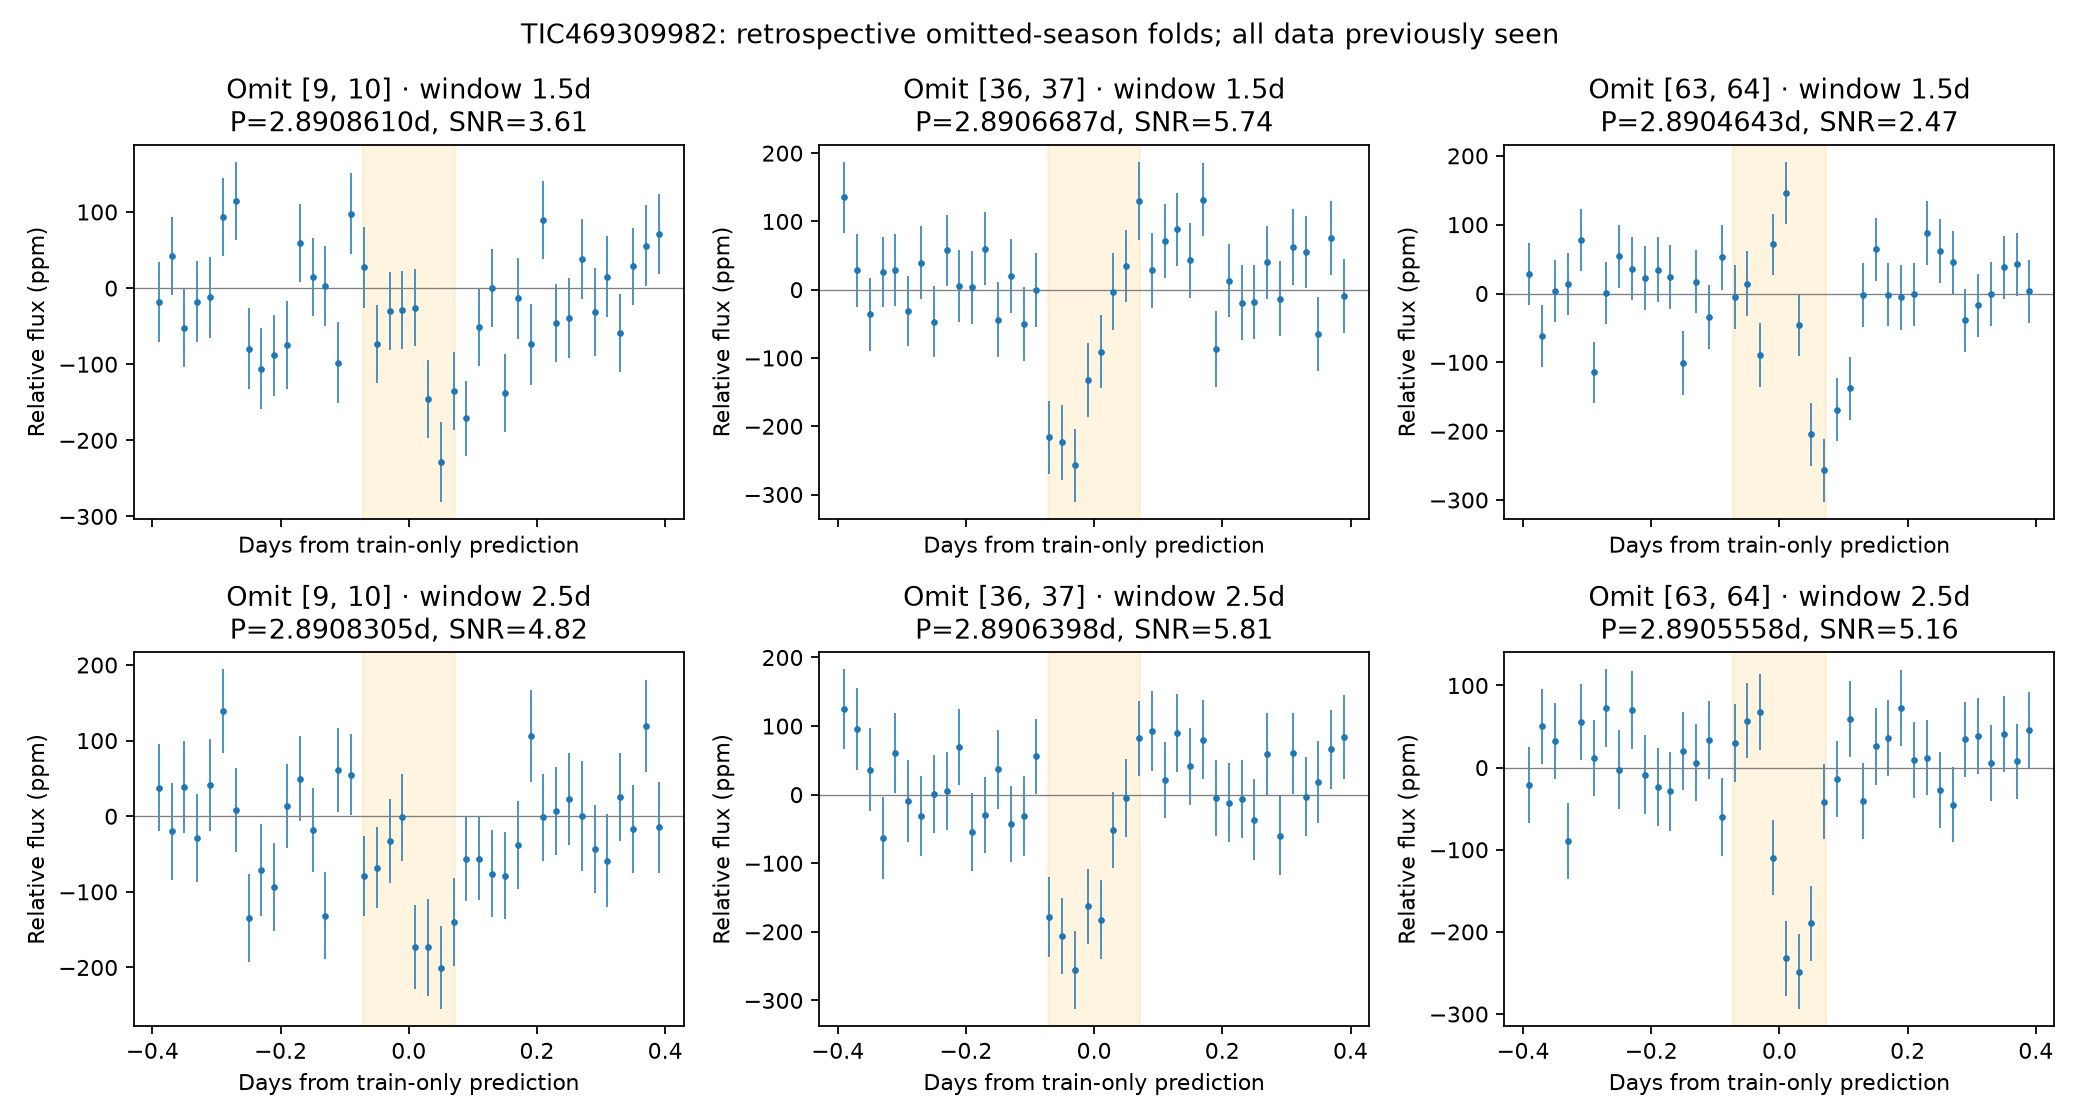
\includegraphics[width=\linewidth]{figures/469-seasons.png}
\caption{Retrospective omitted-season measurements for TIC 469309982.
Columns omit sectors 9/10, 36/37 and 63/64; rows use two detrending windows.
The shaded regions show the predicted boxes. Only the upper middle comparison
passes both timing and recovery gates. The other five remain timing-inconclusive,
including nominally strong lower-row features. All data were already inspected;
the seed and overlapping training sets prevent interpreting these as independent
blind discoveries. Displayed formal signal-to-noise values omit correlated
noise and clock uncertainty.}
\label{fig:469seasons}
\end{figure}

\subsection{TIC 96166003: positive depths depend on the clock}
\label{sec:tic961}
% Evidence: results/review-96166003-20261011/ASSESSMENT.md
% results/expanded-96166003-20261012/ASSESSMENT.md
% results/heldout-96166003-s59-20261012/ASSESSMENT.md

The original sectors 43/44 contain a compact approximately 0.955-day signal,
with fixed-clock local depths near 280~ppm under both detrendings. Sector 19
provides only weak, timing-inconclusive measurements. Once it becomes training,
the expanded primary clock is $P=0.955530474$~d with duration 0.05952~d;
the alternative selects $P=0.955279111$~d and duration 0.048~d. All accepted
profile islands remain preserved.

In sector 59 the primary predicts $264.9\pm51.9$~ppm, whereas the expanded
alternative gives $-72.4\pm62.4$~ppm and the two original-discovery comparisons
also give negative depths. Every prediction fails its timing gate; the primary
spread is 1.34665~d. Crossing both fixed clocks with both detrendings and SAP/
PDCSAP products retains the primary dip and the alternative's near-zero or
negative result. Thus this disagreement follows the timing hypotheses more than
these processing choices, but does not identify the correct hypothesis.

% Evidence: results/new-epochs-469309982-96166003-20261012/ASSESSMENT.md
% results/prf-96166003-20261012/ASSESSMENT.md
New sector 86 gives $248.2\pm100.7$~ppm at the expanded primary and
$7.2\pm134.0$~ppm at its alternative. All six retained comparisons are
low-sensitivity and timing-inconclusive (Figure~\ref{fig:961new}). Discovery
images favor the target nominally, but including faint neighbors changes some
sector-43 rankings. A physically viable diluted-binary alternative remains.
Neither the photometry nor template preferences securely establish a host.
A bibliographic planet-table association is also uninformative.\footnote{The
exact TIC 96166003 row in the checked TESS yield paper describes a simulated
15.592607-day planet, not an observed planet. It neither validates nor
invalidates the approximately 0.955-day signal investigated here.}

% Evidence: results/reliability-469309982-20261012/ASSESSMENT.md
% results/reliability-96166003-20261012/ASSESSMENT.md
For each of these two shallow signals, bounded block controls give zero
exceedances in 40 draws separately for each of three block models. Each
conditional 95\% Monte Carlo interval extends to 8.81\%; counts are not pooled.
These tests condition on selected targets and timing families and cannot supply
survey false-alarm probabilities or planet odds.

\begin{figure}[p]
\centering
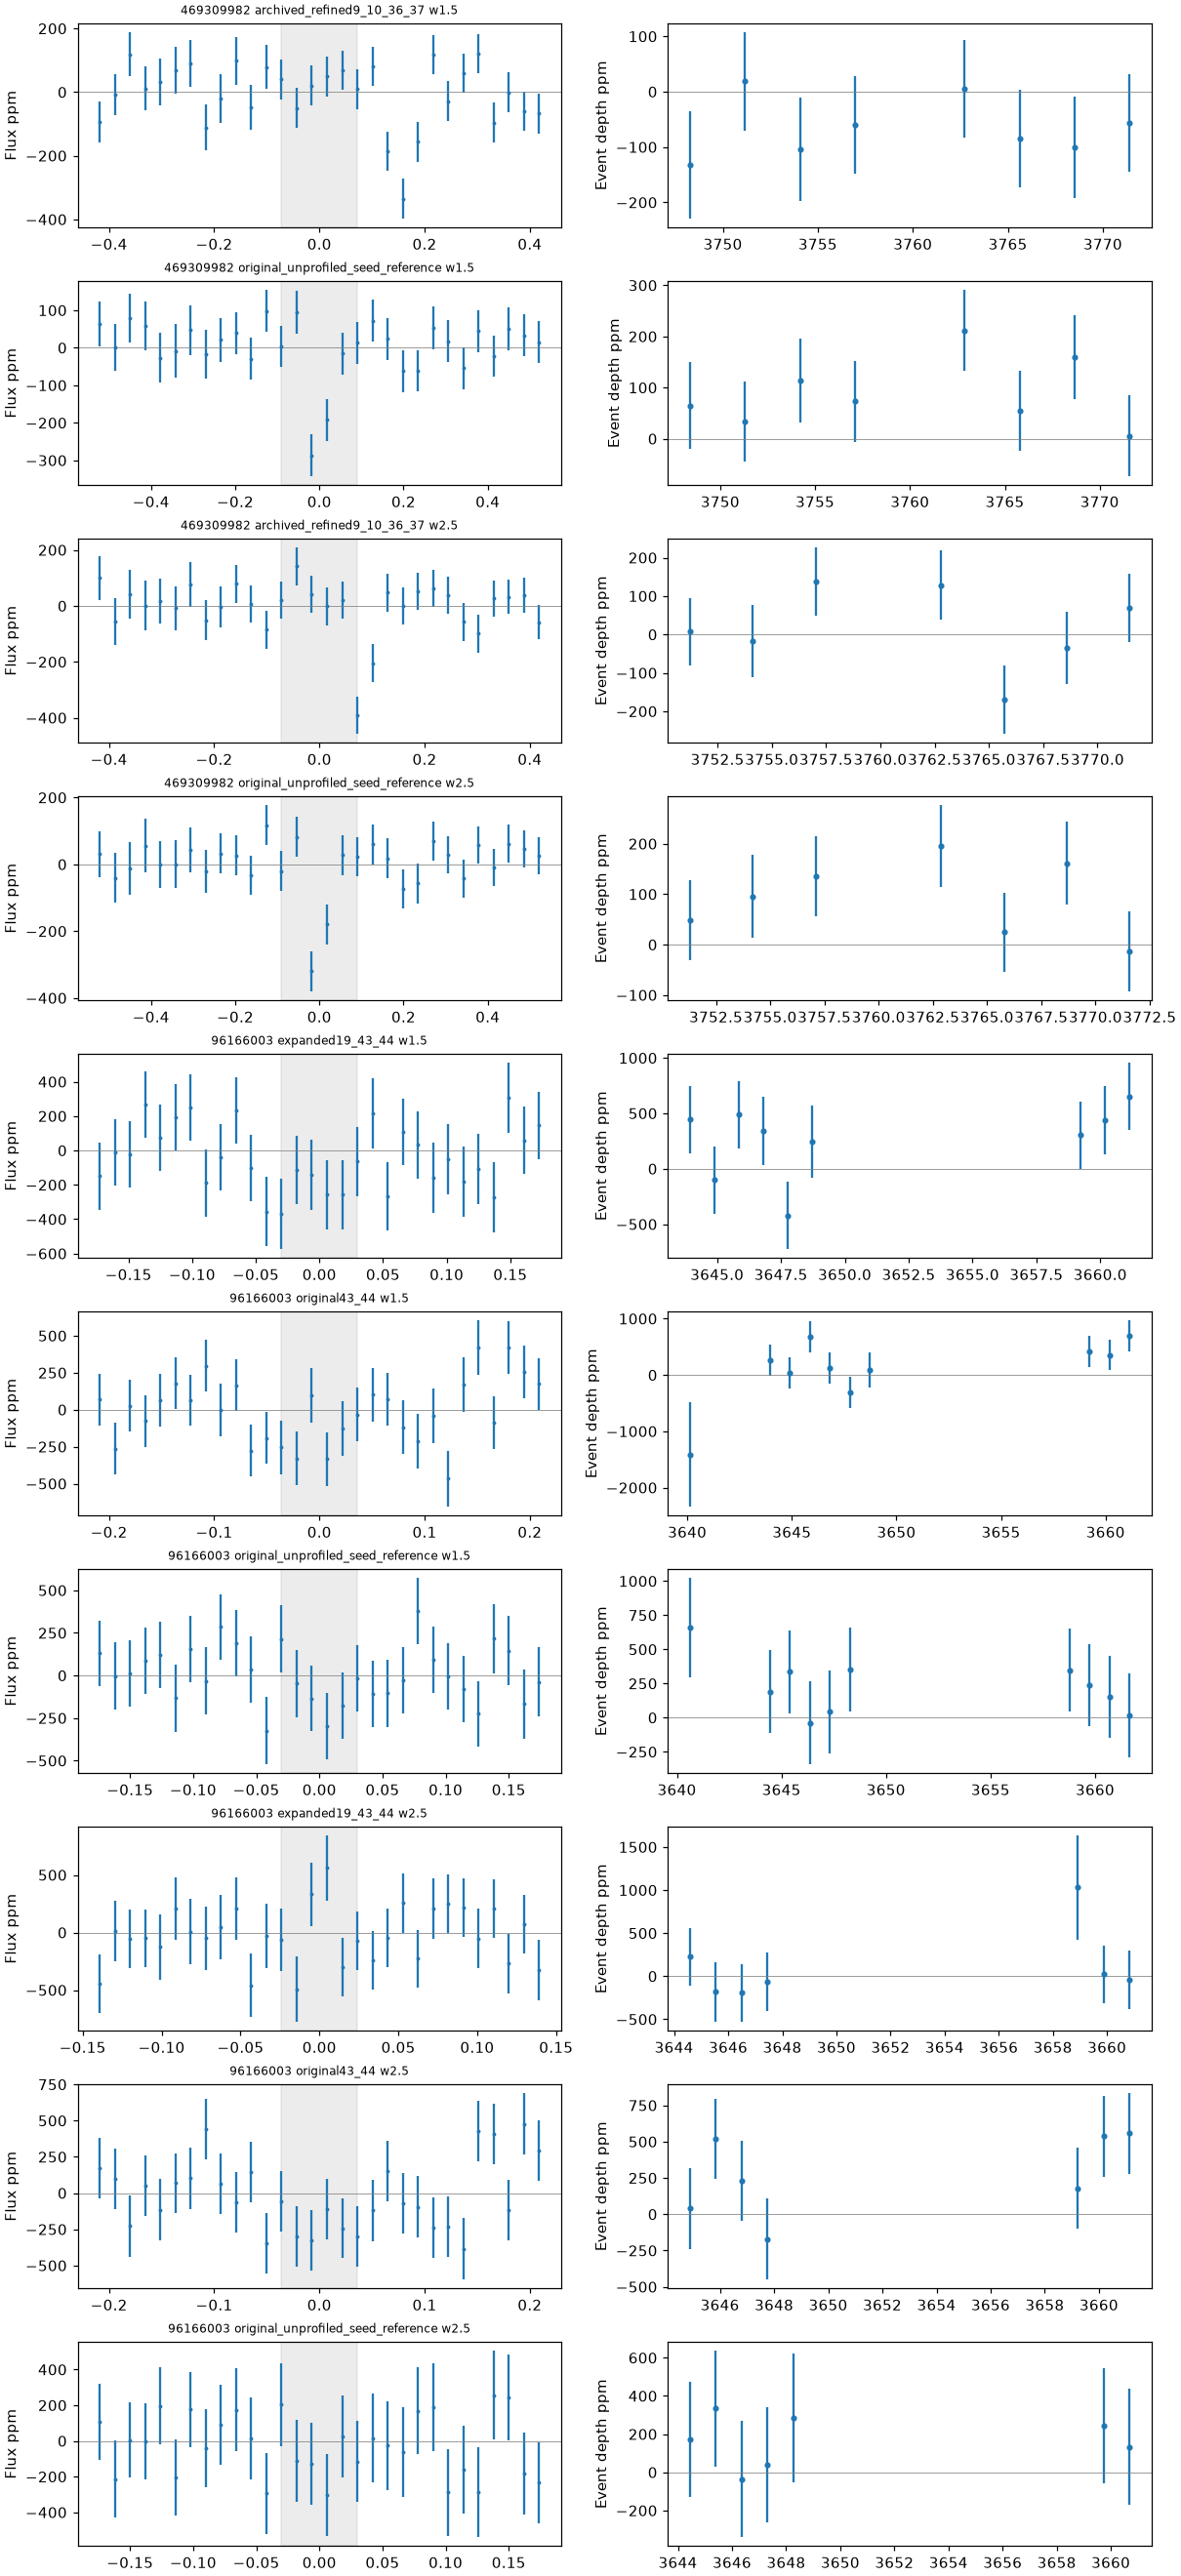
\includegraphics[width=\linewidth,trim=0 1036.8bp 0 0,clip]{figures/469-961-new.png}
\caption{The four saved clock comparisons for TIC 469309982 sector 90.
Left panels show fixed-clock folds (days from the predicted midpoint); right
panels show individual-event depths at centers in BTJD.
Positive depth denotes dimming. The primary result is negative. Profiled
clocks fail timing precision, unprofiled seed references are ineligible for
recovery, and expected formal sensitivity is below $5\sigma$ in every row.
This reproduces the upper four rows of the original ten-row chart; the lower
six rows are shown separately in Figure~\ref{fig:961new} for readability.}
\label{fig:469961new}
\end{figure}

\begin{figure}[p]
\centering
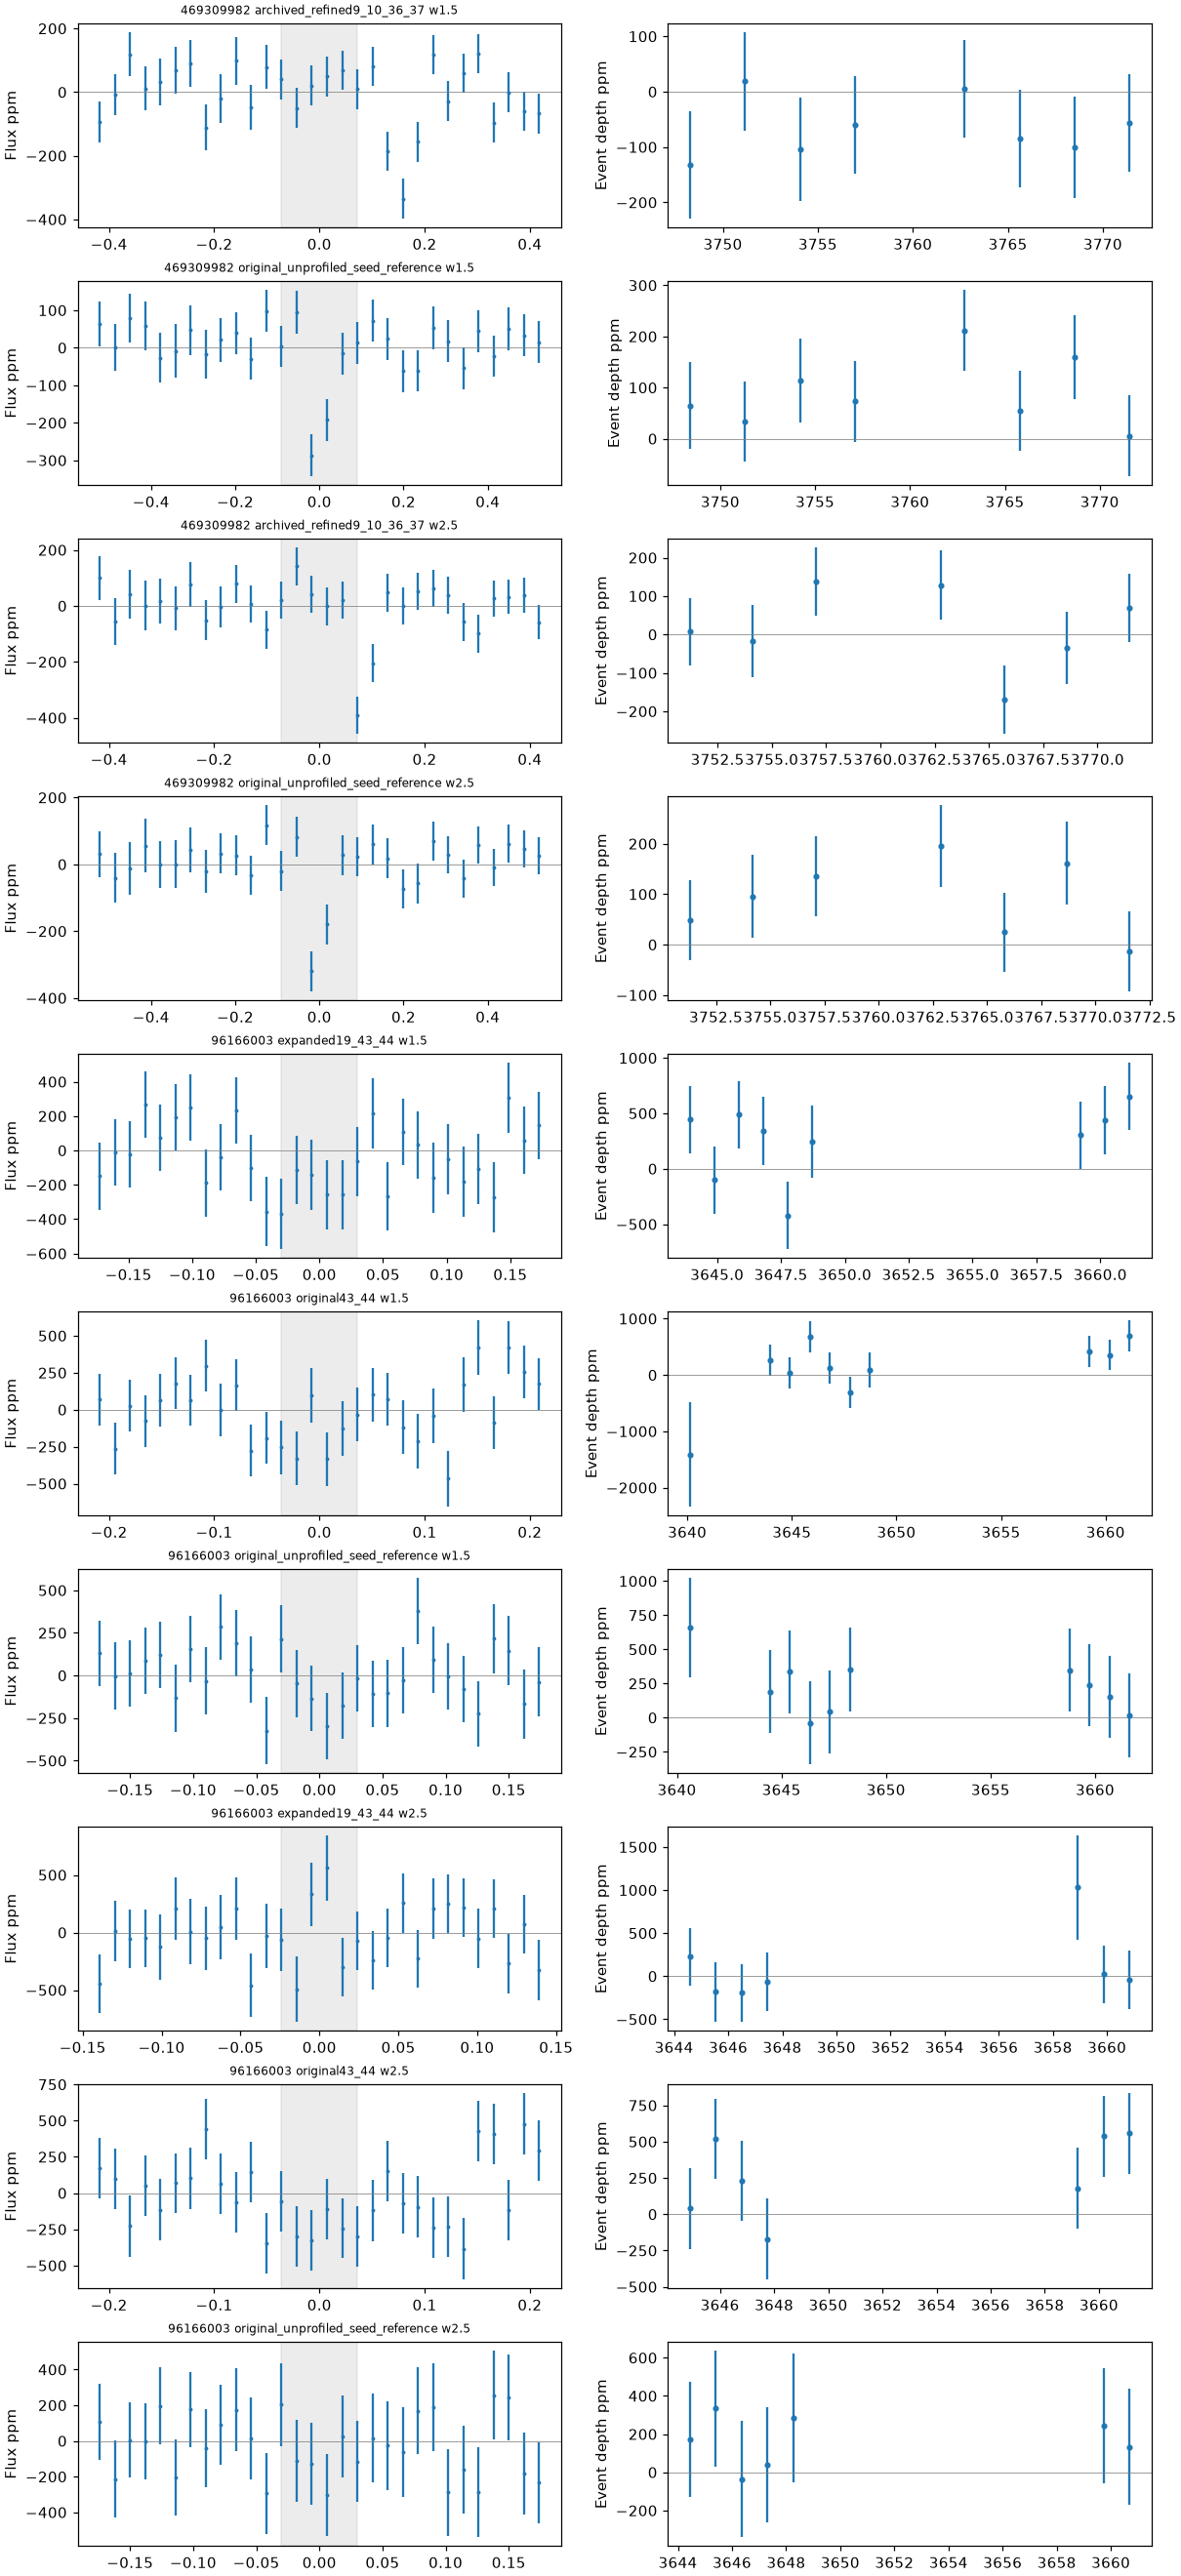
\includegraphics[width=\linewidth,height=0.78\textheight,keepaspectratio,trim=0 0 0 691.2bp,clip]{figures/469-961-new.png}
\caption{The six saved clock comparisons for TIC 96166003 sector 86,
reproducing the lower six rows of the same original chart as
Figure~\ref{fig:469961new}. The primary is weak, and the expanded alternative
is near zero. Left abscissae are days from the predicted midpoint; right
abscissae are event centers in BTJD. Profiled clocks fail timing precision, unprofiled seed references
are ineligible for recovery, and expected formal sensitivity is below
$5\sigma$ in every row. Repeated reductions share photons; none passes the
original recovery requirements. Only page layout has changed.}
\label{fig:961new}
\end{figure}

\subsection{TIC 5546257: resolved-neighbor variability strengthens contamination}
\label{sec:tic554}
% Evidence: results/followup-5546257-20261011/ASSESSMENT.md
% results/new-epochs-5546257-20261012/ASSESSMENT.md

The expanded pre-sector-62 clock, $P=1.767290230$~d and duration 0.133056~d,
gives $386.2\pm30.1$~ppm in sector 62. The timing spread, 0.07203~d, narrowly
exceeds the allowed 0.06653~d. Newly opened QLP sectors 89 and 99 retain nominal
clock dips of $271\pm28$ and $239\pm33$~ppm, but their timing spreads also
fail the original gate. The coarse discovery seed gives negative depths.
Different extraction methods and apertures prevent interpreting these depth
changes as intrinsic evolution or improved source attribution.

% Evidence: results/prf-motion-5546257-s62-20261011/ASSESSMENT.md
% results/contaminant-clock-5546257-20261012/ASSESSMENT.md
Sector-62 source-plus-motion models favor neighboring TIC 5546242:
$\chi^2=259.24/126$, compared with $776.24/126$ for the target. All 13 event
omissions and 10 of 13 individual images favor the neighbor, whose exact Gaia
source is classified as an eclipsing binary. However, its catalog period,
7.248263937 TCB days, and the tested simple harmonics do not explain the
selected TESS train. The closest period division, $P/4=1.812065956$~d, is
2.53\% longer. This mismatch prevents claiming a complete catalog-clock
explanation, while leaving contamination plausible.

% Evidence: results/extension-402358350-5546257-20261012/ASSESSMENT.md
Resolved Gaia epoch photometry of that neighbor supplies stronger adverse
evidence (Figure~\ref{fig:554gaia}). All five nominal in-window measurements
at the unchanged refined TESS clock dim, with relative depth
$16.343\pm0.192\%$; a sixth dim point lies just outside. The backward timing
spread remains too large, and the 13 saved timing alternatives include only
two to six of the conspicuous dim points. The published Gaia model explains
most samples but leaves one notable discrepancy. Sparse sampling permits a
possible catalog alias; no period was refitted to select that explanation.
The neighbor association is strengthened, although its exact orbit, aperture
dilution and quantitative explanation of the TESS signal remain unresolved.

\begin{figure}[p]
\centering
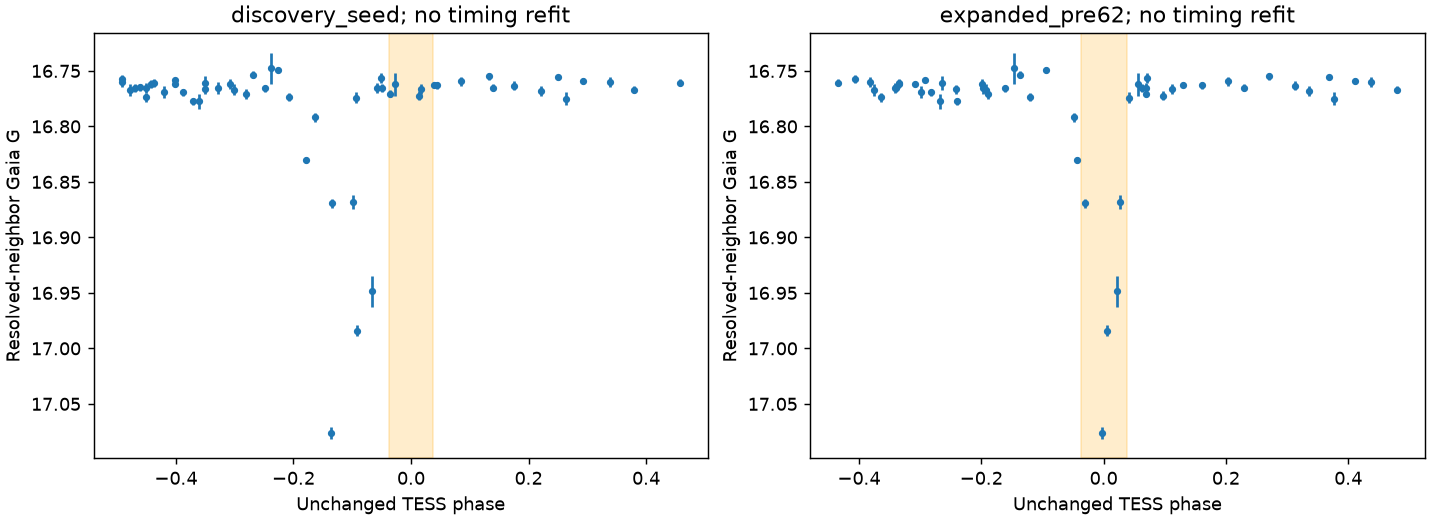
\includegraphics[width=\linewidth]{figures/554-gaia.png}
\caption{Resolved Gaia $G$ measurements of TIC 5546242, the binary neighbor
favored by TIC 5546257 difference images. Left: unchanged coarse discovery
clock. Right: unchanged expanded pre-sector-62 clock. The latter aligns five
dim points within the frozen window and a sixth nearby, supporting
contamination. The backward timing gate still fails, and alternate saved
profiles do not all align the same points. Neither this nominal alignment nor
the catalog model settles the period alias or the TESS dilution. These are
neighbor measurements, not independently confirmed target transits.}
\label{fig:554gaia}
\end{figure}
